\section{Basic Idea}
\subsection{Fallacy: LBA-based Lifetime Prediction}

Current automatic methods predict the lifetime of data based on the update
frequency of LBAs~\cite{AutoStream}.  
For example, AutoStream~\cite{AutoStream} assumes that, if
some LBAs are frequently rewritten by applications, those LBAs hold hot data.
This LBA-based lifetime prediction works poorly on modern applications, where
the majority of new data are written in an append-only manner.  To understand
the correlation between LBAs and the lifetime of data under append-only
workloads, we analyzed the write pattern of RocksDB~\cite{RocksDB}, which is a
popular key-value store based on the LSM-tree algorithm~\cite{LSM}.

Figure~\ref{fig:lba_lifetime}(a) shows the lifetime distribution of data
according to LBAs. Here, the lifetime of data is defined to be 
the number of write requests between when the data is written 
and when the data is invalidated an overwrite or a TRIM command. 
%an elapsed time (unit: $\mu$sec) from when it is newly written to a certain LBA to when it is
%invalidated by an overwrite or a TRIM command. 
As shown in
Figure~\ref{fig:lba_lifetime}(a), there is no strong correlation between the
lifetime and LBAs -- all the data have very different lifetimes, regardless of
their LBA numbers. We also analyzed 
if the lifetimes of LBAs change under some predictable patterns over times 
although the overall lifetime distribution of LBAs shows large variances.
Figure 1(b) shows a scatter plot of data lifetimes over the logical time 
(in the number of write requests) for a 1-MB chunk with 2048 LBAs. 
Over the logical time, the lifetime of data written to the chunk 
varies in an unpredictable fashion.  
For example, at the logical time 10, the lifetime was 1 but it increases about 
2.6 million around the logical time 450 
followed by a rapid drop around the logical time 600. 

Our investigation strongly suggests that  under append-only
workloads, LBAs couldn't be a useful 
indicator that can be used to decide
the hotness or lifetime of data.

\begin{figure}[t]
	\centering
	\subfloat[Lifetime patterns over LBAs]{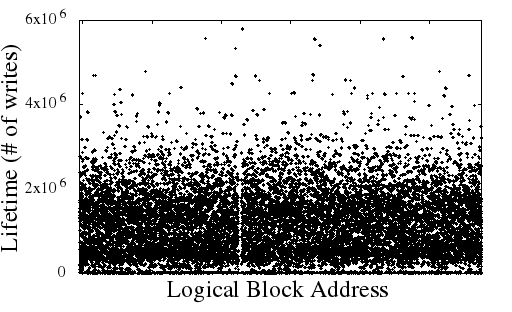
\includegraphics[width=0.25\textwidth]{figure/lba_lifetime2}}  % data from 0/03031641
	\subfloat[Lifetime patterns over time]{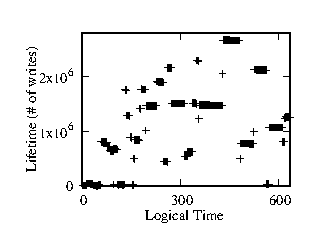
\includegraphics[width=0.22\textwidth]{figure/lifetime_in_chunk2}}
	%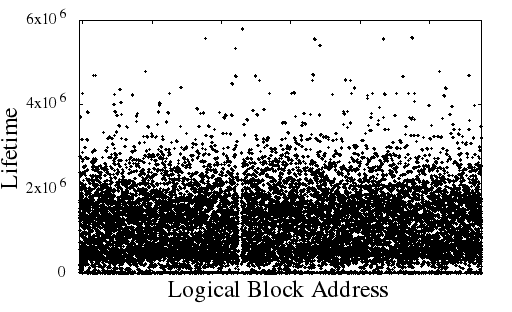
\includegraphics[width=0.9\linewidth]{figure/lba_lifetime} 
	\vspace{-10pt}
	\caption{
		Data lifetime distributions over varying LBAs and logical times.
		\textcolor{red}{(TODO:) it would be good to include same graphs with
		in-place update workloads;}}
		\label{fig:lba_lifetime}
	\vspace{-15pt}
\end{figure}

\subsection{Program Context as a Lifetime Predictor}
In order to separate data with different lifetimes, the key requirement is to devise 
a means with which {\it different I/O contexts} can be effectively distinguished.  
For example, LBAs played such a role fairly well for update workloads.  
However, they do not work well for append-only workloads because 
they do not convey the context of I/O operations any more.  

In developing PCStream, we started from a simple question: 
how can we extract I/O context? 
For example, in RocksDB, logging, flushing and compaction can be regarded
as different I/O contexts.
RocksDB appends write-ahead logs to storage to ensure data
persistence.  Those logs have short lifetimes because they are quickly deleted
(or trimmed) after original data are safely stored in the persistent storage.
The flush module of RocksDB (which materializes the content of a memtable in
DRAM, often called an L0 table, to an L1 table in the storage) generates data
with relatively short lifetimes. This is because an L1 table will be flushed to
an L2 table and be removed in the near future. Conversely, a compaction module
often writes long-lived data that are unlikely to be removed for a long time.

The above observation implies that, if we are able to know the detailed
behaviors of append-only applications, data with different lifetimes can be
isolated in separate streams in an SSD. As mentioned in Section~\ref{sec:intro}, a
common solution~\cite{MultiStream} to realizing this is manually modify an
application code so that each module assigns a unique stream ID to data stream
it generates. However, owing to considerable implementation efforts
required to modify individual applications, this approach is not widely used in
real-world environments.

In this paper, we claim that a program context is a useful tool that delivers
the information of data lifetimes to the storage side without modifying application
code manually. The program context is calculated at runtime by summing the
values of program counters that are identified along function-call paths
of an application. Logging, flushing, and compaction are invoked through
different function-call paths. Thus, by leveraging the program context, we are
able to identify software modules that generate specific write streams. Note
that using the program context to identify characteristics of data is not new.
Ha \textit{et al.} proposed a way of separating hot-cold data by referring to the program
context~\cite{PCHa}. This work, however, was not designed for append-only
applications and didn't take into account the use of a multi-stream feature of
a modern SSD.

\begin{figure}[!t]
\centering
\hspace{1pt}
\subfloat[manual: log]{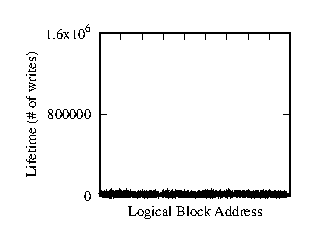
\includegraphics[width=0.23\textwidth]{figure/type_1b}} % data from 4/03031953 
\subfloat[PC\#2]{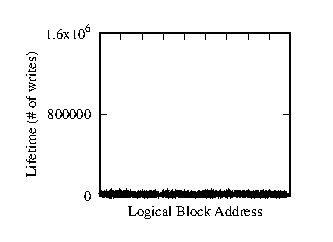
\includegraphics[width=0.23\textwidth]{figure/pcID_2b}}
\hfill
\vspace{-10pt}
\subfloat[manual: flush] {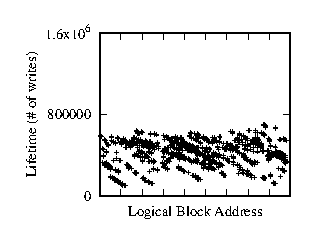
\includegraphics[width=0.23\textwidth]{figure/type_3b}}
\subfloat[PC\#3]{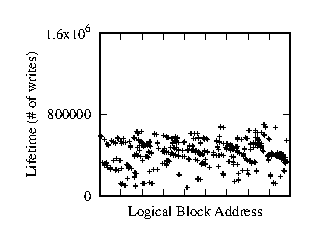
\includegraphics[width=0.23\textwidth]{figure/pcID_3b}}
\caption{Data lifetime distributions of different PCs.} 
\label{fig:types_and_PCs}
\vspace{-20pt}
\end{figure}

In order to confirm our hypothesis that the program context could provide
enough information to recognize detailed behaviors of an application, we
conducted a series of experiments using RocksDB, comparing the accuracy of
lifetime prediction by two different methods: 1) when the type of data streams
is manually identified by modifying the code (\texttt{manual}) and 2) when the
stream type is automatically tagged by the program context
(\texttt{automatic}).  Figure~\ref{fig:types_and_PCs} compares the lifetime
distributions of data that are separated by \texttt{manual} and
\texttt{automatic}.  Figures~\ref{fig:types_and_PCs}(a) and (b) represent how
well the two methods identify log data written by
RocksDB.  As mentioned earlier, log data are short-lived, and the
\texttt{automatic} method with the program context shows high accuracy
comparable to \texttt{manual}. Similarly, Figures~\ref{fig:types_and_PCs}(c)
and (d) shows the accuracy of identifying data streams written by the flush
module of RocksDB.  As expected, these two graphs have the similar lifetime
patterns, which proves that the program context can be a good lifetime hint.


